\documentclass[12pt]{article}
\usepackage{amsfonts}
\usepackage{amsmath}
\usepackage{amsthm}
\usepackage[utf8]{inputenc}
\usepackage{enumitem}
\usepackage{graphicx}
\title{Jawaban UAS Fisika Komputasi (FI-3201) Semester 2 2019-2020}
\author{M Nauval FR 10217023\\
	Steffan RS 10217038\\
	Humam 10217088\\
	Awla FA 10217027\\
	Hans MT 10217045\\
	Wilbert I 10217088\\}
\begin{document}
	\maketitle
	Catatan: selain dibuat dalam format .tex dan pdf, jawaban ini jugua tersedia dalam format .md
% Nomor 01	
\section{Soal No.1}
	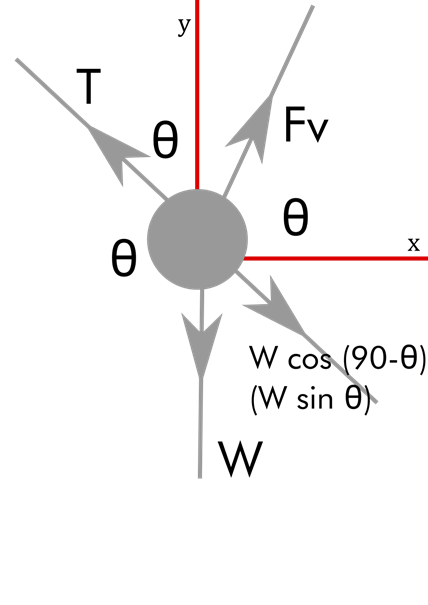
\includegraphics[scale=0.4]{UASFiskom0101.png}\\
	\begin{enumerate}[label=(\alph*)]
		%1a%--------------------------------------------------------------------------------
		\item
		 Didapat persamaan dalam setiap arah gerak bandul sebagai berikut, untuk gerak  sumbu $x$:
		\begin{equation}
		\Sigma F_x = m \ddot{x}
		\end{equation}
		Pertama-tama, dengan melihat gambar dapat ditemukan hubungan
		\begin{equation}
		T \cos \theta -F_{visko_x}= m \ddot{x}
		\end{equation}
		Jika dianalisa gaya searah $\hat{r}$,
		\begin{equation}
		T -\omega sin  \theta= \dfrac{mv^2}{l}
		\end{equation}
		sehingga
		\begin{equation}
		T =\omega sin  \theta + \dfrac{mv^2}{l}
		\end{equation}
		dan
		\begin{equation}
		F_{visko_x}= 3\eta\pi D\ddot{x}.
		\end{equation}
		Jika disubstitusikan,
		\begin{equation}
		-mg \cos\theta \sin\theta+\dfrac{mv^2}{l}cos\theta - 3\pi\eta D \dot{x} -  =m \ddot{x}
		\end{equation}
		Substitusikan persamaan $\cos \theta =\dfrac{x}{l} $ , $\sin \theta =\dfrac{y}{l} $, dan $ w =-mg$, sehingga akan didapat
		\begin{equation}
		\ddot{x} +\dfrac{gxy}{l^2} + \dfrac{3\pi\eta D \dot{x}}{m} -\dfrac{v^2}{l^2}x =0 
		\end{equation} \\
		
		Selanjutnya, akan diturunkan persamaan gerak untuk sumbu y. 
		\begin{equation}
		\Sigma F_y = m \ddot{y}
		\end{equation}
		Dengan melihat gambar, dapat dilihat gaya yang bekerja di sumbu y adalah
		\begin{equation}
		T \sin\theta -mg - F_{visko_y} =m\ddot{y}
		\end{equation}
		Substitusikan persamaan $	F_{visko_y}= 3\eta\pi D\ddot{y}	$ dan $\sin \theta =\dfrac{y}{l} $, sehingga akan didapat
		\begin{equation}
		\ddot{y} + \dfrac{3\pi\eta D}{m} \dot{y} + \dfrac {({\dot{x^2}+\dot{y^2}})y}{l^2} -\dfrac{gy^2}{l^2} = -g
		\end{equation}
		%1b%--------------------------------------------------------------------------------
		\item Untuk persamaan gaya di sumbu x, 
		\begin{equation}
		\dfrac{g}{l^2}xy - \dfrac{3\pi\eta D}{m} \dot{x} - \dfrac{(\dot{x^2}+\dot{y^2})}{l^2}x =\ddot{x}
		\end{equation} \\
		terdapat suku $\ddot{x}$ sebagai komponen percepatan,,$ \dfrac{3\pi\eta D}{m} \dot{x} $ sebagai komponen gaya gesek menggunakan hukum Stokes, $-\dfrac{(\dot{x^2}+\dot{y^2})}{l^2}x$ sebagai komponen gaya sentripetal untuk tegangan tali, dan $\dfrac{g}{l^2}xy$ adalah komponen gaya gravitasi di tegangan tali.
		
		Untuk persamaan gaya di sumbu y, 
		\begin{equation}
		\ddot{y} + \dfrac{3\pi\eta D}{m} \dot{y} + \dfrac {({\dot{x^2}+\dot{y^2}})y}{l^2} -\dfrac{gy^2}{l^2} = -g
		\end{equation}
		terdapat suku $\ddot{y}$ sebagai komponen percepatan,$ \dfrac{3\pi\eta D}{m} \dot{y} $ sebagai komponen gaya gesek menggunakan hukum Stokes, $-\dfrac{(\dot{x^2}+\dot{y^2})}{l^2}y$ sebagai komponen gaya sentripetal untuk tegangan tali, dan $\dfrac{gy^2}{l^2}$ adalah komponen gaya gravitasi di tegangan tali. Selain itu, terdapat juga komponen $-g$ sebagai komponen gravitasi (vertikal sumbu y).
		%1c%--------------------------------------------------------------------------------
		\item 
		Untuk benda jatuh bebas tanpa gesekan udara,  maka persamaan (2) (gaya di sumbu x) berubah menjadi
		\begin{equation}
		\ddot{x} = 0
		\end{equation}
		Persamaan (3) (gaya di sumbu y) berubah menjadi
		\begin{equation}
		\ddot{y} = -g
		\end{equation}
		Saat gaya jatuh bebas tanpa ada gesekan, komponen tegangan dan viskositas bisa diabaikan, sehingga $\eta =0$ dan $ l \approx \infty$.
		%1d%--------------------------------------------------------------------------------
		\item 
		Untuk simpangan kecil, maka $\dfrac{y}{l} \approx 1$ dan $\dfrac{x}{l} \approx \theta$. Tanpa gaya gesek, maka $\eta =0$.
			Sehingga, didapat 
		\begin{equation}
		\ddot{x} - \dfrac{(\dot{x^2}+\dot{y^2})}{l}\theta + g\theta =0
		\end{equation} \\
		\begin{equation}
		\ddot{y} - \dfrac{(\dot{x^2}+\dot{y^2})}{l}\theta + g =-g
		\end{equation}\\
	\end{enumerate}
% nomor 02%--------------------------------------------------------------------------------
\section{Soal No.2}
		\begin{enumerate}[label=(\alph*)]
			%2a%--------------------------------------------------------------------------------
			\item 

			Pertama diketahui posisi bandul sebagai berikut:\\
			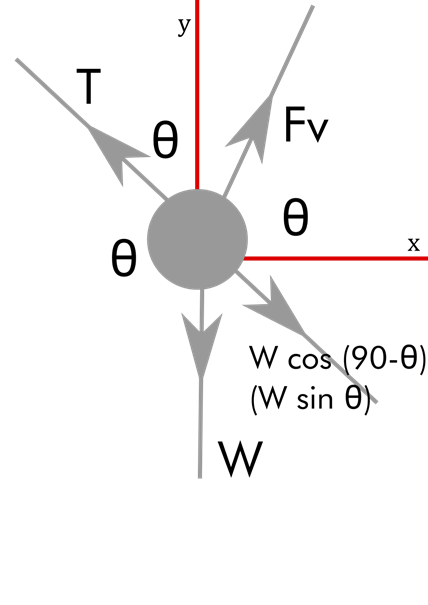
\includegraphics[scale=0.4]{UASFiskom0101.png}\\
			
			T adalah gaya tegang tali, Fv adalah gaya viskositas akibat udara, dan W adalah berat.\\
			Persamaan gerak pada sumbu $\hat{\theta}$ dapat diturunkan dengan mengingat $\alpha = \dfrac{d^2\theta}{dt^2} =\dfrac{M}{I}$, dimana $\alpha$ adalah momentum sudut, M adalah momen, dan I adalah inersia.
			
			Torsi ditentukan oleh proyeksi gaya ke arah tangensial:
			\begin{equation}
			M = -mgL\sin \theta
			\end{equation} 
			Momen inersia pendulum adalah momen inersia lingkaran:
			\begin{equation}
			I = mL^2
			\end{equation} 
			Sehingga, persamaan gerak di sumbu $\hat{\theta}$ adalah, dengan mencoret suku-suku yang sama
			\begin{equation}
			\dfrac{d^2\theta}{dt^2} = \dfrac {M}{I} =\dfrac{g \sin\theta}{L} 
			\end{equation} 
			\begin{equation}
			\dfrac{d^2\theta}{dt^2} +  \dfrac{g  \sin\theta}{L}  =0
			\end{equation} 
			
			Untuk persamaan gerak pada sumbu $ \hat{r}$, berlaku
			\begin{equation}
			\omega \cos \theta +T = \dfrac{mv^2}{r} + m\dot{\theta^2}R
			\end{equation}
			\begin{equation}
			-mg \cos \theta +T = m \dot{\theta^2}l
			\end{equation} 
		\begin{equation}
			 \dot{\theta^2}+\dfrac{g}{l} \cos \theta =\dfrac{T}{ml}
			\end{equation} 
			

			%2b%--------------------------------------------------------------------------------
			\item
			\begin{equation}
			\dfrac{d^2\theta}{dt^2} - \dfrac{g\theta}{l} =0 
			\end{equation} 
			Persamaan diferensial ini adalah persamaan diferensial karakteristik, sehingga  dengan memisalkan $\lambda_{12} = \pm \sqrt{\dfrac{g}{l}}i$, sehingga:
			\begin{equation}
			\theta = C\exp{\lambda_1t}+D\exp{\lambda_2t}
			\end{equation} 
			\begin{equation}
			\theta = C (\cos \sqrt{\dfrac{g}{l}}t + i \sin \sqrt{\dfrac{g}{l}}t) +D(\cos \sqrt{\dfrac{g}{l}}t - i \sin \sqrt{\dfrac{g}{l}}t)
			\end{equation} 
			\begin{equation}
			\theta = (C+D) \cos \sqrt{\dfrac{g}{l}}t +  i (C-D) \sin \sqrt{\dfrac{g}{l}}t
			\end{equation} 		
			\begin{equation}
			\theta = A \cos \sqrt{\dfrac{g}{l}}t +   B \sin \sqrt{\dfrac{g}{l}}
			\end{equation} 	
			Saat t = 0, asumsikan bandul berada di amplitudo ($\theta_{max}$) sehingga sudut maksimum.
			\begin{equation}
			\theta_{max} = A \cos 0 + 0 \Rightarrow \theta_{max} = A
			\end{equation} 	
			Didapat A = amplitudo, B  = 0.
			Sehingga, pada akhirnya akan didapat 
			\begin{equation}
			\theta = A \cos  \sqrt{\dfrac{g}{l}}t, \\ \dot{\theta} =-\sqrt{\dfrac{g}{l}} A \sin \sqrt{\dfrac{g}{l}}t
			\end{equation} 	
			Untuk persamaan kedua, dengan mensubstitusikan persamaan sebelumnya,
			\begin{equation}
			\dot{\theta^2} + \dfrac{g}{l}cos\theta = \dfrac{T}{lm}
			\end{equation} 
			Karena menggunakan pendekatan sudut kecil, maka	
			\begin{equation}
			T \approx \left((\sqrt{\dfrac{g}{l}}A\sin \sqrt{\dfrac{g}{l}}t)^2 +\sqrt{\dfrac{g}{l}}\cos\theta\right)lm
			\end{equation} 	
			\begin{equation}
			T \approx A^2 g \sin^2 (\sqrt{\dfrac{g}{l}}t) +m\sqrt{gl}  \cos \theta
			\end{equation} 
			Hasil dari perhitungan menggunakan metode analitik digrafikkan di 			
			\begin{verbatim} https://plotly.com/~Avestory/3/#/
			\end{verbatim}
				
			%2c%--------------------------------------------------------------------------------
			\item Dengan metode Euler,
			\begin{equation}
			\dfrac{df}{dx}= \dfrac{f(x+L)-f(x)}{h} \Rightarrow \dfrac{f^{i+1}-f^i}{\Delta x}
			\end{equation}
			Persamaan $\ddot{\theta}$ dan $\dot{\theta}$ dapat dirubah menjadi
		\begin{equation}
			\dot{\theta}=\dfrac{d\theta}{dt}=  \dfrac{\theta^{i+1}-\theta^i}{\Delta t} \Rightarrow \theta^{i+1} = \dot{\theta}^i\Delta t+ \theta^i
			\end{equation}
			dan
			\begin{equation}
			\ddot{\theta}=\dfrac{g}{l} \sin \theta \Rightarrow  \dfrac{d\dot{\theta}^i}{dt} =  \dfrac{g}{l} \sin \theta
			\end{equation}
			\begin{equation}
		 \dfrac{\dot{\theta}^{i+1}-\dot{\theta}^i}{\Delta t} = \dfrac{g}{l} \sin \theta^{i} 
			\end{equation}
			\begin{equation}
			\theta^{i+1}=\dfrac{g}{l} \sin \dot{\theta}^{i}\Delta t+\dot{\theta}^i 
			\end{equation}
			Hasil dari perhitungan menggunakan metode numerik digrafikkan di 			\begin{verbatim}https://plotly.com/~Avestory/1/#/
			\end{verbatim}
			
			%2d%--------------------------------------------------------------------------------
			\item 
			Untuk menyelesaikan secara numerik, dibuat kode di C++ sebagai berikut:
			\begin{verbatim}
			#include <iostream>
			#include <cmath>
			#include <fstream>
			
			using namespace std;
			
			int main(){
			/* variabel yang digunakan */
			float g,l,h,m,tt;
			int i,n;
			
			g = 9.82;
			
			/*besar panjang tali*/
			l=1;
			/*besar massa*/
			m=0.5;
			/*total waktu analisis*/
			tt = 10;
			/*step waktu yang digunakan*/
			h = 0.1;
			
			n = tt/h;
			float theta[n],thetadot[n],f[n],T[n],t[n];
			
			for (i=0;i<n;i++){
			t[i] = 0;
			f[i] = 0;
			T[i] = 0;
			theta[i] = 0;
			thetadot[i] = 0;
			}
			
			/* pendefinisian awal */
			theta[0] = 30*3.14/180;
			thetadot[0] = 0;
			
			/* logika euler dan input data yang didapat ke file theta.txt */
			ofstream myfile;
			myfile.open ("theta.txt");
			for (i=0; i<=n; i++){
			theta[i+1] = theta[i] + thetadot[i]*h;
			f[i] = (g/l)*sin(theta[i+1])*-1;
			thetadot[i+1] = thetadot[i] + f[i]*h;
			T[i] = l*m*(thetadot[i]*thetadot[i] + g*cos(theta[i])/l);
			
			t[i+1] = t[i] + h;
			
			myfile <<  t[i]  << "  "  << theta[i] << "  " << thetadot[i] << "  " << T[i] << "\n";
			
			cout << "t[" << i << "]: " << t[i] << "\n";
			cout << "theta[" << i << "]: " << theta[i] << "\n";
			cout << "thetadot[" << i << "]: " << thetadot[i] << "\n";
			cout << "T[" << i << "]: " << T[i] << "\n" << "\n";
			}
			myfile.close();
			
			
			/* terminasi program */
			return 0;
			}
			\end{verbatim}
			Kode juga akan disertakan di GitHub \\ (https://github.com/mnauvalfr/uasfiskom/blob/master/kodeno2d.cpp) dan CPPSH (cpp.sh/2ybae)
		\end{enumerate}
% nomor 03
\section{Soal No.3}
\begin{enumerate}[label=(\alph*)]
	\item %3a
	Dalam proses penyelesaian masalah, dataset yang telah diberikan dimasukkan terlebih dahulu ke dalam perangkat lunak Microsoft Excel untuk dianalisa bentuk persebaran datanya. Untuk tabel data pertama, terdapat persebaran data seperti berikut.\\
	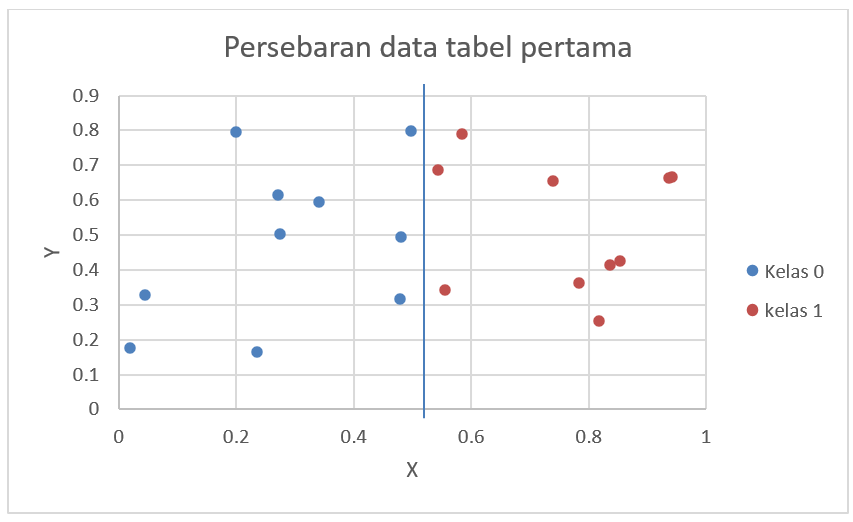
\includegraphics[scale=1]{UASFiskom0301.png}\\
	Berdasarkan persebaran data yang terdapat di tabel di atas, terlihat jelas bahwa data dapat dipisahkan dengan metode perceptron. Dengan data yang telah didapatkan, dilakukan uji coba di laman daring Artificial Neural Network Playground yang disediakan oleh Tensorflow. Ketentuan dan batasan uji coba yang terdapat adalah sebagai berikut. 
	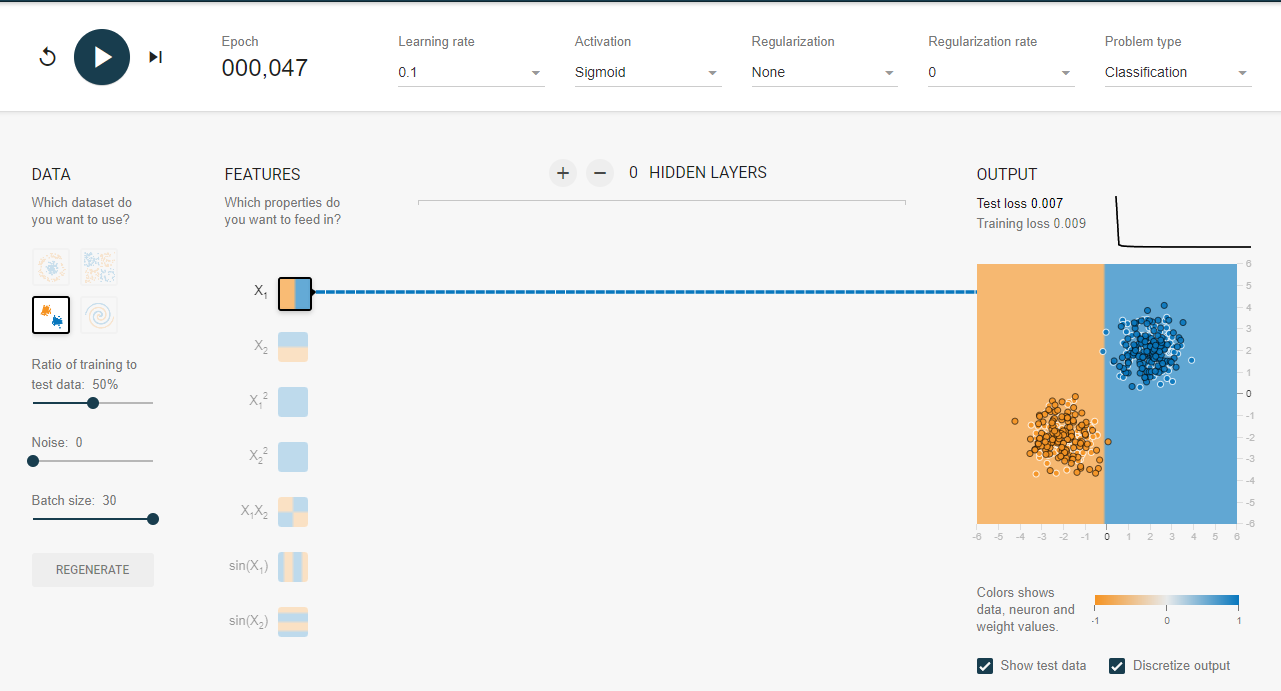
\includegraphics[scale=0.4]{UASFiskom0302.png}\\
	Berdasarkan data persebaran yang ada, dataset yang paling mirip dengan persebaran yang sudah dirumuskan adalah dataset yang dipilih. Ditentukan hanya satu neuron input karena dataset yang perlu dianalisa memiliki dua fitur di mana hanya satu fitur yang berkontribusi terhadap pembagian kelas (N1=1). Hidden layer tidak digunakan pada uji coba ini karena berdasarkan persebaran data, data dapat dipisah menggunakan linear boundary. Tanpa hidden layer yang mengandung satu neuron, dapat dilihat bahwa hanya dalam 47 iterasi (epoch), data sudah secara rapi terpisah. Sehingga, arsitektur yang digunakan pada dataset ini adalah 1-0-1.
	\item %3b
	Dalam proses penyelesaian masalah, dataset yang telah diberikan dimasukkan terlebih dahulu ke dalam perangkat lunak Microsoft Excel untuk dianalisa bentuk persebaran datanya. Untuk tabel data pertama, terdapat persebaran data seperti berikut.\\
	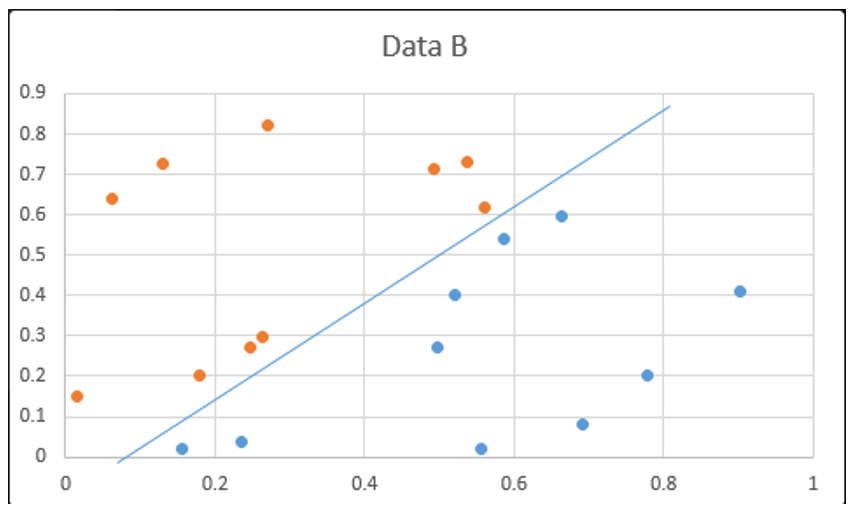
\includegraphics[scale=1]{UASFiskom0303.png}\\
	Berdasarkan persebaran data yang terdapat di tabel di atas, terlihat jelas bahwa data dapat dipisahkan dengan metode perceptron. Dengan data yang telah didapatkan, dilakukan uji coba di laman daring Artificial Neural Network Playground yang disediakan oleh Tensorflow. Ketentuan dan batasan uji coba yang terdapat adalah sebagai berikut. \\
	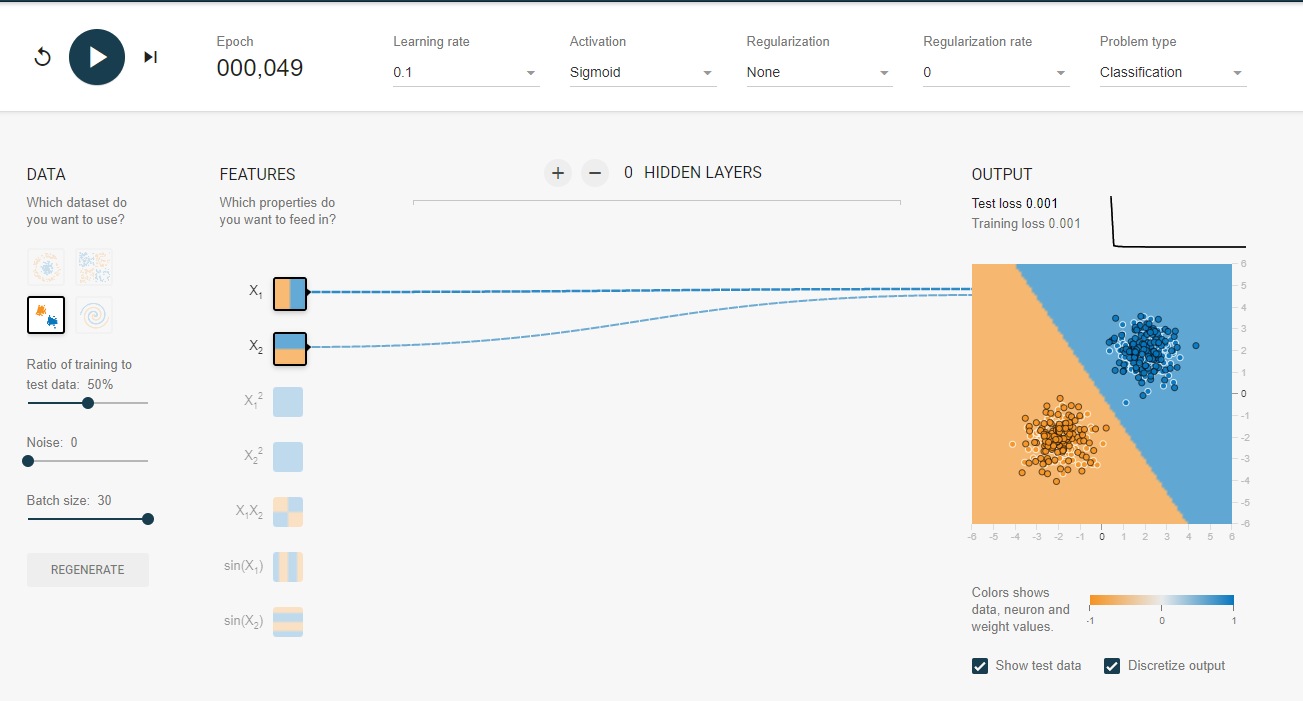
\includegraphics[scale=0.4]{UASFiskom0304.png}\\
	Berdasarkan data persebaran yang ada, dataset yang paling mirip dengan persebaran yang sudah dirumuskan adalah dataset yang dipilih. Ditentukan dua neuron input karena dataset yang perlu dianalisa memiliki dua fitur (N1=2). Hidden layer tidak digunakan pada uji coba ini karena berdasarkan persebaran data, data dapat dipisah menggunakan linear boundary. Tanpa hidden layer yang mengandung satu neuron, dapat dilihat bahwa hanya dalam 49 iterasi (epoch), data sudah secara rapi terpisah. Sehingga, arsitektur yang digunakan pada dataset ini adalah 2-0-1.
	\item %3c
	Untuk penentuan JST, akan lebih mudah jika terlebih dahulu divisualisasikan. Pertama, data yang diperoleh dimasukkan pada perangkat lunak Excel dan diurutkan outputnya agar terpisah data yang memberikan output kelas 0 dan 1. Kemudian, dibuat diagram scatter dengan warna output 1 dan 0 berbeda dengan Excel dan ditarik garis boundary layer agar bisa ditentukan berapa boundary layer yang dibutuhkan. \\
	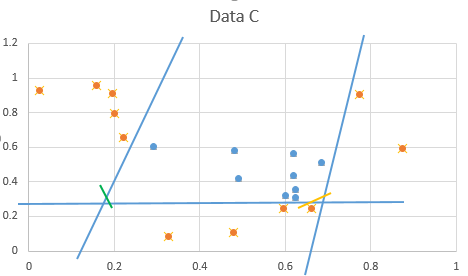
\includegraphics[scale=1]{UASFiskom0305.png}\\
	Dari gambar ini terlihat garis memiliki kemiringan artinya sumbu x dan sumbu y keduanya ikut berpengaruh terhadap hasil. Sehingga, bisa disimpulkan bahwa layer input yang digunakan adalah 2 yaitu fitur x dan y (N1=2).
	Dari gambar terlihat dibutuhkan minimal 3 boundary layer, jumlah boundary setara dengan jumlah neuron yang dibutuhkan hidden layer sehingga untuk hidden layer N2 dibutuhkan minimal 3 neuron untuk memisahkan. Agar training lebih cepat, untuk hidden layer N2, neuron dapat ditambah satu untuk menghaluskan boundary seperti diberikan oleh garis kuning sedangkan garis hijau diwakili oleh output layer. Tetapi, untuk kesederhanaan ANN maka sebenarnya cukup digunakan tiga neuron pada satu hidden layer (N2=3).
	Dari gambar, terlihat bahwa output yang diharapkan adalah pemisah yaitu 1 dan 0 sehingga bentuk output layer hanya memisahkan 2 data diskrit. Maka, output layer hanya memerlukan 1 yaitu pemisah 1 dan 0 (N3 = 1).
	Didapat N1 - N2 - N3 = 2 – 3 – 1.
	\item %3d
	Penjelasan sebenarnya sudah dijelaskan dari 3.a hingga 3.c., didapatkan dari visualisasi dataset pertama bahwa data terpisah secara jelas oleh satu garis sehingga diperlukan dua neuron input untuk dua fitur x dan y dan karena pemisah linear, maka tidak diperlukan hidden layer. Untuk dataset kedua, dipisahkan oleh garis miring sehingga kedua sumbu x dan y berpengaruh sehingga diperlukan dua neuron input. Tetapi, karena masih bisa dipisahkan boundary linear maka tidak dimerlukan hidden layer. Sedangkan, untuk data C, diperlukan dua input dan pemisah harus diwakili oleh 3 boundary sehingga diperlukan satu hidden layer dengan tiga neuron.
	Arsitektur JST yang sederhana penting karena semakin rumit arsitektur maka iterasi yang dilakukan semakin lama dan panjang serta resource yang diperlukan juga meningkat. Kita harus seefisien mungkin dalam mengalokasikan computational resource terutama jika yang akan diolah data yang besar.
	
\end{enumerate}
\section{Soal No.4}
\begin{enumerate}[label=(\alph*)]
	\item 
	Kode yang dibuat adalah dengan input kromoson 0010110
	\begin{verbatim}
		main();
		// Define main function
		function main() {
		var p = "0010110";
		[xs, ys, cs] = getValues(p);
		console.log("p =",p);
		console.log("x =",xs);
		console.log("y =",ys);
		console.log("c =",cs);
		}
		function getValues() {
		var p = arguments[0];
		var xs = p.slice(0, 3);
		var ys = p.slice(3, 6);
		var cs = p.slice(6);
		
		return [xs, ys, cs];
		}
	\end{verbatim}
	Hasil yang diperoleh adalah sebagai berikut:\\
	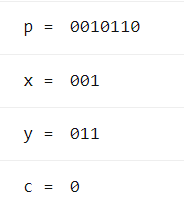
\includegraphics[scale=1]{UASFiskom0401.png}\\
	Kode yang sama dapat juga diakses di GitHub dan dapat dijalankan secara daring menggunakan jsconsole.com.
	\item
	Fungsi \textit{fitness} yang diminta dibuat dalam kode berikut, dengan $x_0$ =111 dan $y_0$=111.
	\begin{verbatim}
	main();
	// Define main function
	function main() {
	var p = "1010110";
	[xs, ys, cs] = getValues(p);
	var hasil = 1/(1+fitness(xs,ys));			//fungsi utuh fitting
	console.log("p =",p);
	console.log("x =",xs);
	console.log("y =",ys);
	console.log("c =",cs);
	console.log("hasil = ",hasil);
	}
	
	function getValues() {
	var p = arguments[0];
	var xs = p.slice(0, 3);
	var ys = p.slice(3, 6);
	var cs = p.slice(6);
	return [xs, ys, cs];
	}
	
	\end{verbatim}

	Kode yang sama dapat juga diakses di GitHub dan dapat dijalankan secara daring menggunakan jsconsole.com.
  \item 
  Kode yang dibuat dengan nilai x0 adalah 111 dan y0 adalah 111.
  	\begin{verbatim}
  	main();
  	
  	
  	//
  	// Define main function 
  	function main() 
  	{ var p = "1010110";
  	var q = "1011111";
  	var r = "1111011";
  	var s = "1110110";
  	var t = "1111101";
  	var threshold= 0.5;
  	[x1, y1, c1] = getValues(p); 
  	[x2, y2, c2] = getValues(q); 
  	[x3, y3, c3] = getValues(r); 
  	[x4, y4, c4] = getValues(s); 
  	[x5, y5, c5] = getValues(t); 
  	var hasil1 = 1/(1+fitness(x1,y1));
  	var seleksi1 = selection(threshold, hasil1, p)
  	console.log("p =",p); 
  	console.log("x =",x1); 
  	console.log("y =",y1); 
  	console.log("c =",c1);
  	console.log("hasil = ",hasil1);
  	console.log("seleksi = ",p," ",  seleksi1);
  	var hasil2 = 1/(1+fitness(x2,y2));
  	var seleksi2 = selection(threshold, hasil2, q)
  	console.log("q =",q); 
  	console.log("x =",x2); 
  	console.log("y =",y2); 
  	console.log("c =",c2); 
  	console.log("hasil = ",hasil2);
  	console.log("seleksi = ",q," ",  seleksi2);
  	var hasil3 = 1/(1+fitness(x3,y3));
  	var seleksi3 = selection(threshold, hasil3, r)
  	console.log("r =",r); 
  	console.log("x =",x3); 
  	console.log("y =",y3); 
  	console.log("c =",c3); 
  	console.log("hasil = ",hasil3);
  	console.log("seleksi = ",r," ",  seleksi3);
  	var hasil4 = 1/(1+fitness(x4,y4));
  	var seleksi4 = selection(threshold, hasil4, s)
  	console.log("s =",s); 
  	console.log("x =",x4); 
  	console.log("y =",y4); 
  	console.log("c =",c4); 
  	console.log("hasil = ",hasil4);
  	console.log("seleksi = ",s," ", seleksi4);
  	var hasil5 = 1/(1+fitness(x5,y5));
  	var seleksi5 = selection(threshold, hasil5, t)
  	console.log("t =",t); 
  	console.log("x =",x5); 
  	console.log("y =",y5); 
  	console.log("c =",c5); 
  	console.log("hasil = ",hasil5);
  	console.log("seleksi = ",t," ", seleksi5);
  	}
  	
  	function getValues() 
  	{ var p = arguments[0];
  	var xs = p.slice(0, 3); 
  	var ys = p.slice(3, 6); 
  	var cs = p.slice(6);
  	return [xs, ys, cs]; 
  	}
  	function fitness(a, b) 
  	{ return(Math.sqrt(Math.pow((a - 111), 2) + Math.pow((b - 111),2))); 
  	}
  	
  	function selection(threshold, a, p)
  	{ if (a>=threshold) { result="pass the selection";
  	} else { result="didnt pass the selection";
  	}
  	return (result);
  	}
  	\end{verbatim}
  	Hasil yang diperoleh adalah sebagai berikut:\\
  	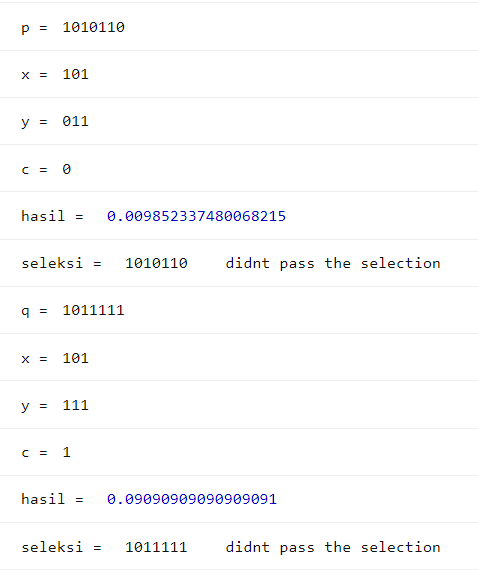
\includegraphics[scale=1]{UASFiskom0402.png}\\
  	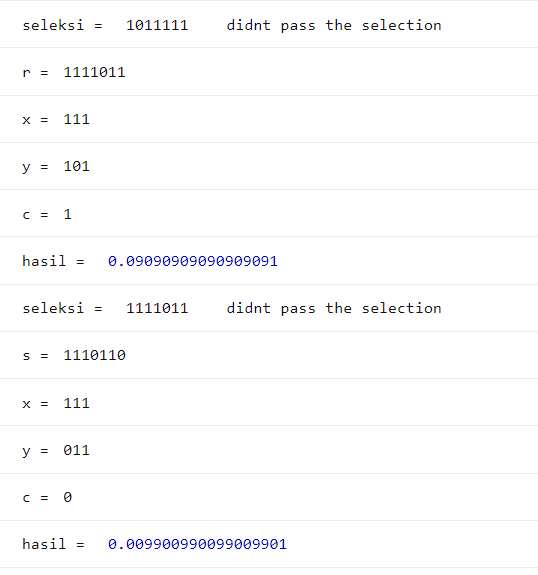
\includegraphics[scale=1]{UASFiskom0403.png}\\
  	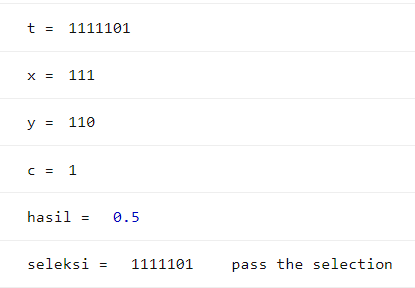
\includegraphics[scale=1]{UASFiskom0404.png}\\
  	Kode yang sama dapat juga diakses di GitHub dan dapat dijalankan secara daring menggunakan jsconsole.com.
  	\item Kode yang dipakai sama dengan kode untuk nomor 4b, dengan x0 =101, y0 =100.
  	  	\begin{verbatim}
  	main();
  	
  	// Define main function
  	function main() {
  	var p = "1011001";    //input kromoson yang diuji
  	[xs, ys, cs] = getValues(p);
  	var hasil = 1/(1+fitness(xs,ys));
  	console.log("p =",p);
  	console.log("x =",xs);
  	console.log("y =",ys);
  	console.log("c =",cs);
  	console.log("hasil = ",hasil);
  	
  	}
  	
  	function getValues() {
  	var p = arguments[0];
  	
  	var xs = p.slice(0, 3);
  	var ys = p.slice(3, 6);
  	var cs = p.slice(6);
  	
  	return [xs, ys, cs];
  	}
  	
  	function fitness(a, b) {
  	return(Math.sqrt(Math.pow((a - 101), 2) + Math.pow((b - 100),2)));	//ganti nilai dalam akar untuk kromoson referensi
  	}
  	
  	\end{verbatim}
  	Kromoson yang akan di-check adalah \\
  	•	1111011 , x = 111 dan y = 101\\
  	  	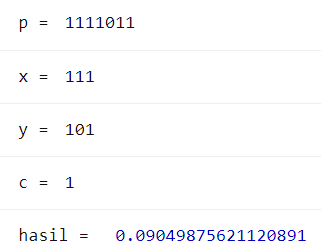
\includegraphics[scale=1]{UASFiskom0405.png}\\
  	•	1001111 , x = 100 dan y = 111\\
  	  	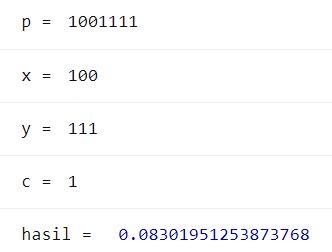
\includegraphics[scale=1]{UASFiskom0406.png}\\
  	•	1001001, x = 100 dan y = 100\\
  	  	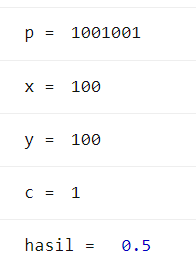
\includegraphics[scale=1]{UASFiskom0407.png}\\
  	•	1111111, x = 111 dan y = 111\\
  	  	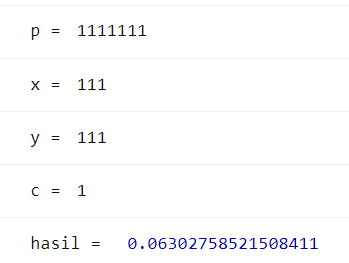
\includegraphics[scale=1]{UASFiskom0408.png}\\
  	•	1011001, x = 101 dan y = 100\\
	  	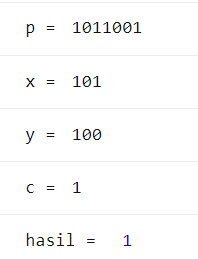
\includegraphics[scale=1]{UASFiskom0409.png}\\
  	
  	Hasil maksimal yang diperoleh adalah kromoson 1011001 karena sama dengan kromoson threshold dengan fitness 1 dan kromoson yang paling mendekati 1011001 adalah kromoson 1001001 dengan nilai fitness 0,5 dari 5 iterasi yang dicoba.
  	
	\end{enumerate}

\section{Soal No.5}
	\begin{enumerate}
		\item Tujuan\\
		Salah satu pemanfaatan terbaik untuk fisika komputasi adalah dalam analisis desain dan data reaktor nuklit
		Tujuan dari analisis desain dan data nuklir adalah menentukan performa sebuah reaktor nuklir ,yang ditentukan oleh beberapa variabel. Dalam RBL ini, yang dibahas hanya dua, yaitu fluks sumber neutron dan daya reaktor.

		\item Rumusan Masalah \\
		-Bagaimana grafik distribusi flux neutron suatu sumber reaktor silinder?
		
		-Berapa daya reaktor?
		\item Usulan Metode \\
		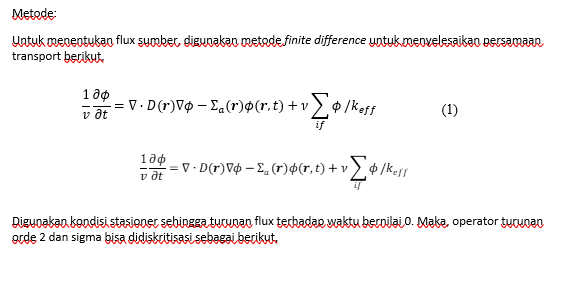
\includegraphics[scale=1]{UASFiskom0501.png}\\
		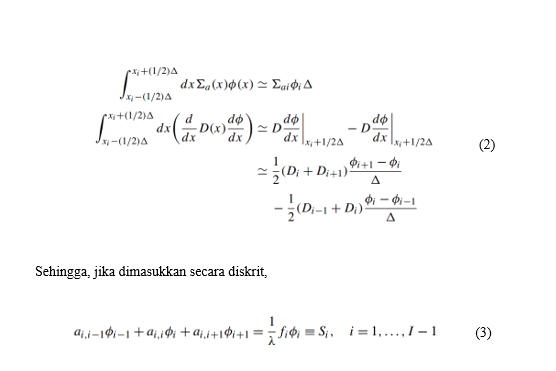
\includegraphics[scale=1]{UASFiskom0502.png}\\
		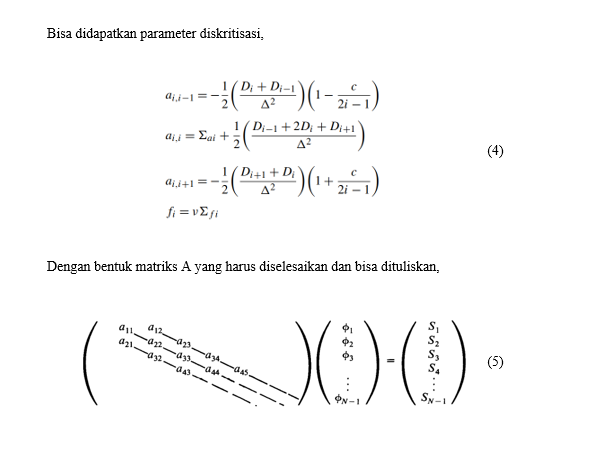
\includegraphics[scale=1]{UASFiskom0503.png}\\
		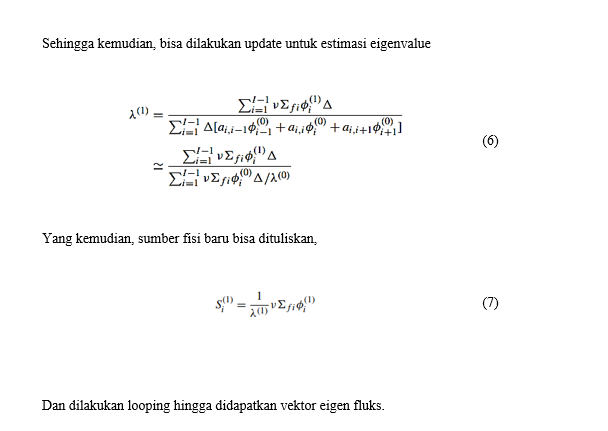
\includegraphics[scale=1]{UASFiskom0504.png}\\
		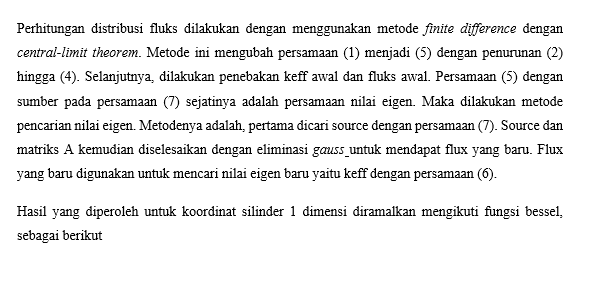
\includegraphics[scale=1]{UASFiskom0505.png}\\
		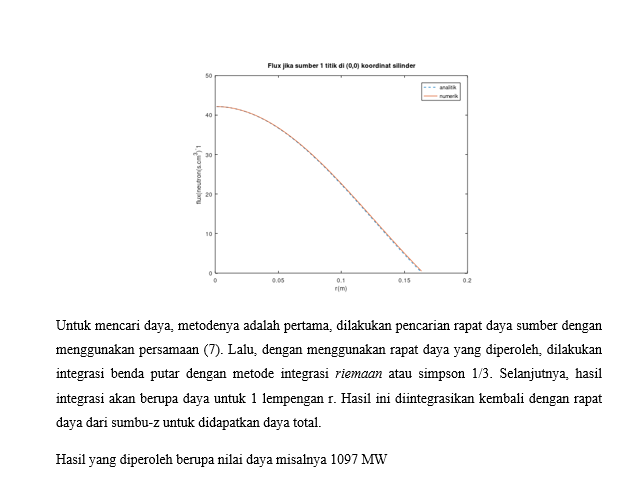
\includegraphics[scale=1]{UASFiskom0506.png}\\
		\item Prakiraan hasil dan analisis \\
		Hasil dari pencarian fluks adalah distribusi fluks, Keff (koefisien pengali neutorn efektif) awal, dan fluks awal. Perhitungan fluks sangat penting untuk menentukan performa reaktor nuklir, salah satunya adalah daya. Flux yang dihasilkan akan turun mengikuti fungsi bessel. 
		Sementara itu, hasil perhitungan daya adalah nilai numerik.
		\item Referensi\\
		1.Ding, Zechuan.(2018). Solving Bateman Equation for Xenon Transient Analysis Using Numerical Methods.
		
		2. Duderstadt, J. and Hamilton, L. (1976). Nuclear Reactor Analysis. New York: Wiley and Sons.
		
		3. Stacey, Weston M. (2018). Nuclear Reactor Physics. 3rd ed. Wiley.
		
	\end{enumerate}
\end{document}
%--------------------------------------------------------------------------------